
% This LaTeX was auto-generated from MATLAB code.
% To make changes, update the MATLAB code and republish this document.

\documentclass{article}
\usepackage{graphicx}
\usepackage{color}

\sloppy
\definecolor{lightgray}{gray}{0.5}
\setlength{\parindent}{0pt}

\begin{document}

    
    
\subsection*{Contents}

\begin{itemize}
\setlength{\itemsep}{-1ex}
   \item Unknown Input Observer Dynamic Simulation for a car suspension system
   \item Step one: Check rank
   \item Step two: Compute Observer Matricies
   \item Step three: check observability
   \item Simulation results
   \item Sim the system
   \item Plot the results
\end{itemize}


\subsection*{Unknown Input Observer Dynamic Simulation for a car suspension system}

\begin{par}
Please see the associated ShareLaTeX pdf file "UIO and Examples"
\end{par} \vspace{1em}
\begin{verbatim}
%----System Physical Constants----%
mb = 300;    % kg
mw = 60;     % kg
bs = 1000;   % N/m/s
ks = 16000 ; % N/m
kt = 190000; % N/m

% --------System Matrices(It is a SIMO system)---------%
A = [ 0 1 0 0; [-ks -bs ks bs]/mb ; ...
      0 0 0 1; [ks bs -ks-kt -bs]/mw]
B = [0 0; 0 10000/mb ; 0 0; [kt -10000]/mw]
C = eye(4)
%D = [0 0; 0 0; B(2,:)];

%---------Disturbance Matrix----------%
E=[1;1;1;1]

%---------LQR design----------%
Q=[.25 0 0 0;0 4 0 0;0 0 1 0;0 0 0 4]
R=50*eye(2)
[K1 l s]=lqr(A,B,Q,R)
\end{verbatim}

        \color{lightgray} \begin{verbatim}
A =

   1.0e+03 *

         0    0.0010         0         0
   -0.0533   -0.0033    0.0533    0.0033
         0         0         0    0.0010
    0.2667    0.0167   -3.4333   -0.0167


B =

   1.0e+03 *

         0         0
         0    0.0333
         0         0
    3.1667   -0.1667


C =

     1     0     0     0
     0     1     0     0
     0     0     1     0
     0     0     0     1


E =

     1
     1
     1
     1


Q =

    0.2500         0         0         0
         0    4.0000         0         0
         0         0    1.0000         0
         0         0         0    4.0000


R =

    50     0
     0    50


K1 =

   -0.2843    0.1013    0.2801    0.2780
   -0.0239    0.1782    0.2067   -0.0136


l =

   12.4869   -0.0583   -4.9018   -0.0045
   -0.0583    0.2753    0.3322    0.0016
   -4.9018    0.3322   17.7047    0.0044
   -0.0045    0.0016    0.0044    0.0044


s =

   1.0e+02 *

  -8.9328 + 0.0000i
  -0.0632 + 0.0581i
  -0.0632 - 0.0581i
  -0.0260 + 0.0000i

\end{verbatim} \color{black}
    

\subsection*{Step one: Check rank}

\begin{par}
We check to see if the rank(CE) = rank(E) = 1
\end{par} \vspace{1em}
\begin{verbatim}
rank(C*E)
rank(E)
\end{verbatim}

        \color{lightgray} \begin{verbatim}
ans =

     1


ans =

     1

\end{verbatim} \color{black}
    

\subsection*{Step two: Compute Observer Matricies}

\begin{par}
Since we have no issues in the previous step, let us compute the observer matrices now:
\end{par} \vspace{1em}
\begin{verbatim}
H = E*inv((C*E)'*(C*E))*(C*E)'
T = eye(4)-H*C
A1 = T*A

f=zeros(4,4)
v=[-4 -4 -4 -4]
F=diag(v)

k1=inv(C)*(A-F-H*C*A)
k2=F*H
k=zeros
k=k1+k2
\end{verbatim}

        \color{lightgray} \begin{verbatim}
H =

    0.2500    0.2500    0.2500    0.2500
    0.2500    0.2500    0.2500    0.2500
    0.2500    0.2500    0.2500    0.2500
    0.2500    0.2500    0.2500    0.2500


T =

    0.7500   -0.2500   -0.2500   -0.2500
   -0.2500    0.7500   -0.2500   -0.2500
   -0.2500   -0.2500    0.7500   -0.2500
   -0.2500   -0.2500   -0.2500    0.7500


A1 =

   1.0e+03 *

   -0.0533   -0.0026    0.8450    0.0031
   -0.1067   -0.0069    0.8983    0.0064
   -0.0533   -0.0036    0.8450    0.0041
    0.2133    0.0131   -2.5883   -0.0136


f =

     0     0     0     0
     0     0     0     0
     0     0     0     0
     0     0     0     0


v =

    -4    -4    -4    -4


F =

    -4     0     0     0
     0    -4     0     0
     0     0    -4     0
     0     0     0    -4


k1 =

   1.0e+03 *

   -0.0493   -0.0026    0.8450    0.0031
   -0.1067   -0.0029    0.8983    0.0064
   -0.0533   -0.0036    0.8490    0.0041
    0.2133    0.0131   -2.5883   -0.0096


k2 =

    -1    -1    -1    -1
    -1    -1    -1    -1
    -1    -1    -1    -1
    -1    -1    -1    -1


k =

     0


k =

   1.0e+03 *

   -0.0503   -0.0036    0.8440    0.0021
   -0.1077   -0.0039    0.8973    0.0054
   -0.0543   -0.0046    0.8480    0.0031
    0.2123    0.0121   -2.5893   -0.0106

\end{verbatim} \color{black}
    

\subsection*{Step three: check observability}

\begin{par}
We must check the system A1,C observability
\end{par} \vspace{1em}
\begin{verbatim}
rank(obsv(A1,C))
\end{verbatim}

        \color{lightgray} \begin{verbatim}
ans =

     4

\end{verbatim} \color{black}
    

\subsection*{Simulation results}

\begin{par}
Set up simulation initial condiditons
\end{par} \vspace{1em}
\begin{verbatim}
X_0 = [-1;10;3;5]
\end{verbatim}

        \color{lightgray} \begin{verbatim}
X_0 =

    -1
    10
     3
     5

\end{verbatim} \color{black}
    

\subsection*{Sim the system}

\begin{verbatim}
sim('car_sus')
plot(X),hold on,plot(Xhat,'--')
\end{verbatim}

        \color{lightgray} \begin{verbatim}Warning: Output port 1 of 'car_sus/Outside Signals' is not connected. 
Warning: Output port 2 of 'car_sus/Outside Signals' is not connected. 
Warning: Output port 3 of 'car_sus/Outside Signals' is not connected. 
Warning: Input port 1 of 'car_sus/Plant' is not connected. 
Warning: Input port 2 of 'car_sus/Plant' is not connected. 
Warning: Input port 3 of 'car_sus/Plant' is not connected. 
Warning: Input port 3 of 'car_sus/UIO/Sum4' is not connected. 
Warning: Using a default value of 0.06 for maximum step size.  The simulation
step size will be equal to or less than this value.  You can disable this
diagnostic by setting 'Automatic solver parameter selection' diagnostic to
'none' in the Diagnostics page of the configuration parameters dialog 
\end{verbatim} \color{black}
    
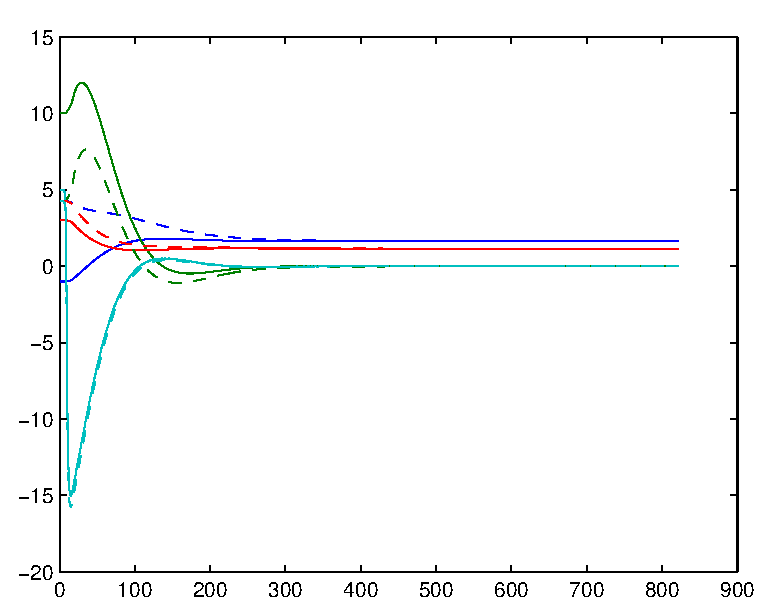
\includegraphics [width=4in]{carsus_01.eps}


\subsection*{Plot the results}

\begin{par}
t = linspace(1,10,length(X\_hat)); figure(1),plot(t,X),hold on plot(t,X\_hat(:,1),'xb'),hold on plot(t,X\_hat(:,2),'xg'),hold on plot(t,X\_hat(:,3),'xr') xlabel('Time in seconds'),ylabel('State trajectory and estimate') title('Dynamic system state and UIO estimate') legend('x\_1','x\_2','x\_3','x\_1 hat','x\_2 hat','x\_3 hat')
\end{par} \vspace{1em}
\begin{verbatim}
% %------Design of bank UIOs each insensitive to One  sensor Fault-----%
%
% %----UIO-1---%
% k11=k1;
% H1=zeros(4,4);
% H1(1:4,2:4)=.25;
% C1=C;
% C1(:,1)=0;
% T1=eye(4)-H1*C1;
% F1=T1*A-k11*C1;
% k12=F1*H1;
% K1=k11+k12;
%
% %----UIO-2----%
% k21=k1;
% H2=zeros(4,4);
% H2(1:4,[1,3,4])=.25;
% C2=C;
% C2(:,2)=0;
% T2=eye(4)-H2*C2;
% F2=T2*A-k21*C2;
% k22=F2*H2;
% K2=k21+k22;
%
% %----UIO-3----%
% k31=k1;
% H3=zeros(4,4);
% H3(1:4,[1,2,4])=.25;
% C3=C;
% C3(:,3)=0;
% T3=eye(4)-H3*C3;
% F3=T3*A-k31*C3;
% k32=F3*H3;
% K3=k31+k32;
%
% %---UIO-4----%
% k41=k1;
% H4=zeros(4,4);
% H4(1:4,1:3)=.25;
% C4=C;
% C4(:,4)=0;
% T4=eye(4)-H4*C4;
% F4=T4*A-k41*C4;
% k42=F4*H4;
% K4=k41+k42;
\end{verbatim}



\end{document}
    
